

\tikzstyle{e0}[0]=[dotted,bend right=#1]
\tikzstyle{e1}[0]=[solid, bend left =#1]
\defmath\hv{{\hat v}}

\tikzset{every node/.style={initial text={}, inner sep=2pt, outer sep=0}}

\section{The \limdd data structure}
\label{sec:isomorphism-qmdd}


\begin{wrapfigure}{r}{7cm} 
%\begin{figure}
\vspace{-2.5em}
\begin{empheq}[box={\Garybox[Domains of variables]}]{align*}
%\begin{align*}
%\Aboxed{
%\tikzmark{A}
    n, i , j, k                 &\in \mathbb N          && \text{indices} \\
    v, w,u                      &\in \Node     && \text{\limdd nodes}\\
    e, f                           &\in \Edge     && \text{\limdd edges}\\
    L, M                        &\in \textnormal{DD} && \limdd \text{(diagrams)} \\ 
    \ket\phi, \ket\psi                  &\in \mathbb C^{\otimes n}  && \text{$n$-qubit states}\\
    \alpha, \beta, \lambda,\mu  &\in \mathbb C          && \text{complex factors}\\
    P, Q, R                     &\in \Pauli^{\otimes n}&& \text{\pauli strings}\\
    A, B                        &\in \mathbb C \times  \Pauli^{\otimes n}
                                      & & \text{Pauli LIMs}~~~~~~~
%\tikzmark{B}
%}
\end{empheq}
%\tikz[remember picture,overlay]\draw(A.north west)rectangle(B.south east);
%\end{figure}
\vspace{-1em}
\end{wrapfigure}

%The figure on the right lists the default domains of variables used in this paper.

Where \qmdds only merge nodes representing the same state up to a constant factor, the \limdd data structure goes further by also merging nodes that are equivalent up to local operations, called Local Invertible Maps (LIMs) (see \autoref{def:isomorphism}).
As a result, \limdds can be exponentially more succinct than \qmdds, including some stabilizer states (see \autoref{sec:exponential-separations}).
    We will call nodes which are equivalent under LIMs, \emph{(LIM-) isomorphic}.
This definition generalizes SLOCC equivalence; in particular, if we choose the parameter $G$ to be the linear group, then the two notions coincide (Appendix A of \cite{dur2000three})~\cite{bennett1996concentrating,chitambar2014everything}.


\begin{definition}[LIM, Isomorphism]
	\label{def:isomorphism}
    A $n$-qubit Local Invertible Map (LIM) is an operator $\mathcal{O}$ of the form $\mathcal{O}=\lambda \mathcal{O}_n\otimes\cdots\otimes \mathcal{O}_1$, where the matrices $\mathcal{O}_i$ are invertible $2\times 2$ matrices and $\lambda\in\mathbb{C}\setminus \{0\}$.
    An \emph{isomorphism} between two $n$-qubit quantum states $\ket{\phi},\ket{\psi}$ is a LIM $\mathcal{O}$ such that $\mathcal{O}\ket{\phi} = \ket{\psi}$.
    If $G$ is a group of $2\times 2$ invertible matrices and if all $\mathcal{O}_i \in G$, then we say that $\mathcal{O}$ is a $G$-isomorphism and that  $\ket{\phi}$ is $G$-isomorphic to $\ket{\psi}$, denoted $\ket{\phi}\simeq_G\ket{\psi}$.
\end{definition}


Before we give the formal definition of \limdds in \autoref{def:limdd}, we give a motivating example in Figure~\ref{fig:qmdd-isoqmdd-exposition} which demonstrates how the use of isomorphisms can yield small diagrams for a four-qubit state.
%Here a $4$-qubit state is represented in four different ways.
In the state's \qmdd, the nodes $c_3$ and $c_4$ represent the two-qubit state vectors $\ket{c_3}=\left[1,1,1,-1  \right]^\dagger$ and $\ket{c_4}=\left[1,-1,\omega,-\omega  \right]^\dagger$.
By noticing that these two vectors are related via $\ket{c_4}=(T\otimes Z)\ket{c_3}$, we may discard the node $c_4$ and store the isomorphism $T\otimes Z$ instead.
%The state $\ket{c_4}$ can then be recovered from $\ket{c_3}$ by computing $\ket{c_4}=(T\otimes Z)\ket{c_3}$.
% todo LV: ze hebben allemaal andere isomorphisms.
In fact, all the nodes on the \qmdd's third level (i.e., the grandchildren nodes of the root node) are related to each other through such isomorphisms.
A similar reduction in size can be achieved at the \qmdd's second level, by noticing that nodes $c_1$ and $c_2$ are related via $\ket{c_2}=Z\otimes I\otimes Z\ket{c_1}$.
The resulting data structure is a \limdd of only five nodes instead of ten.
\autoref{sec:exponential-separations} shows that discarding isomorphic nodes sometimes leads to exponentially smaller diagrams, while the additional cost of storing the isomorphisms is only polynomial.

\begin{figure}[bh!]
	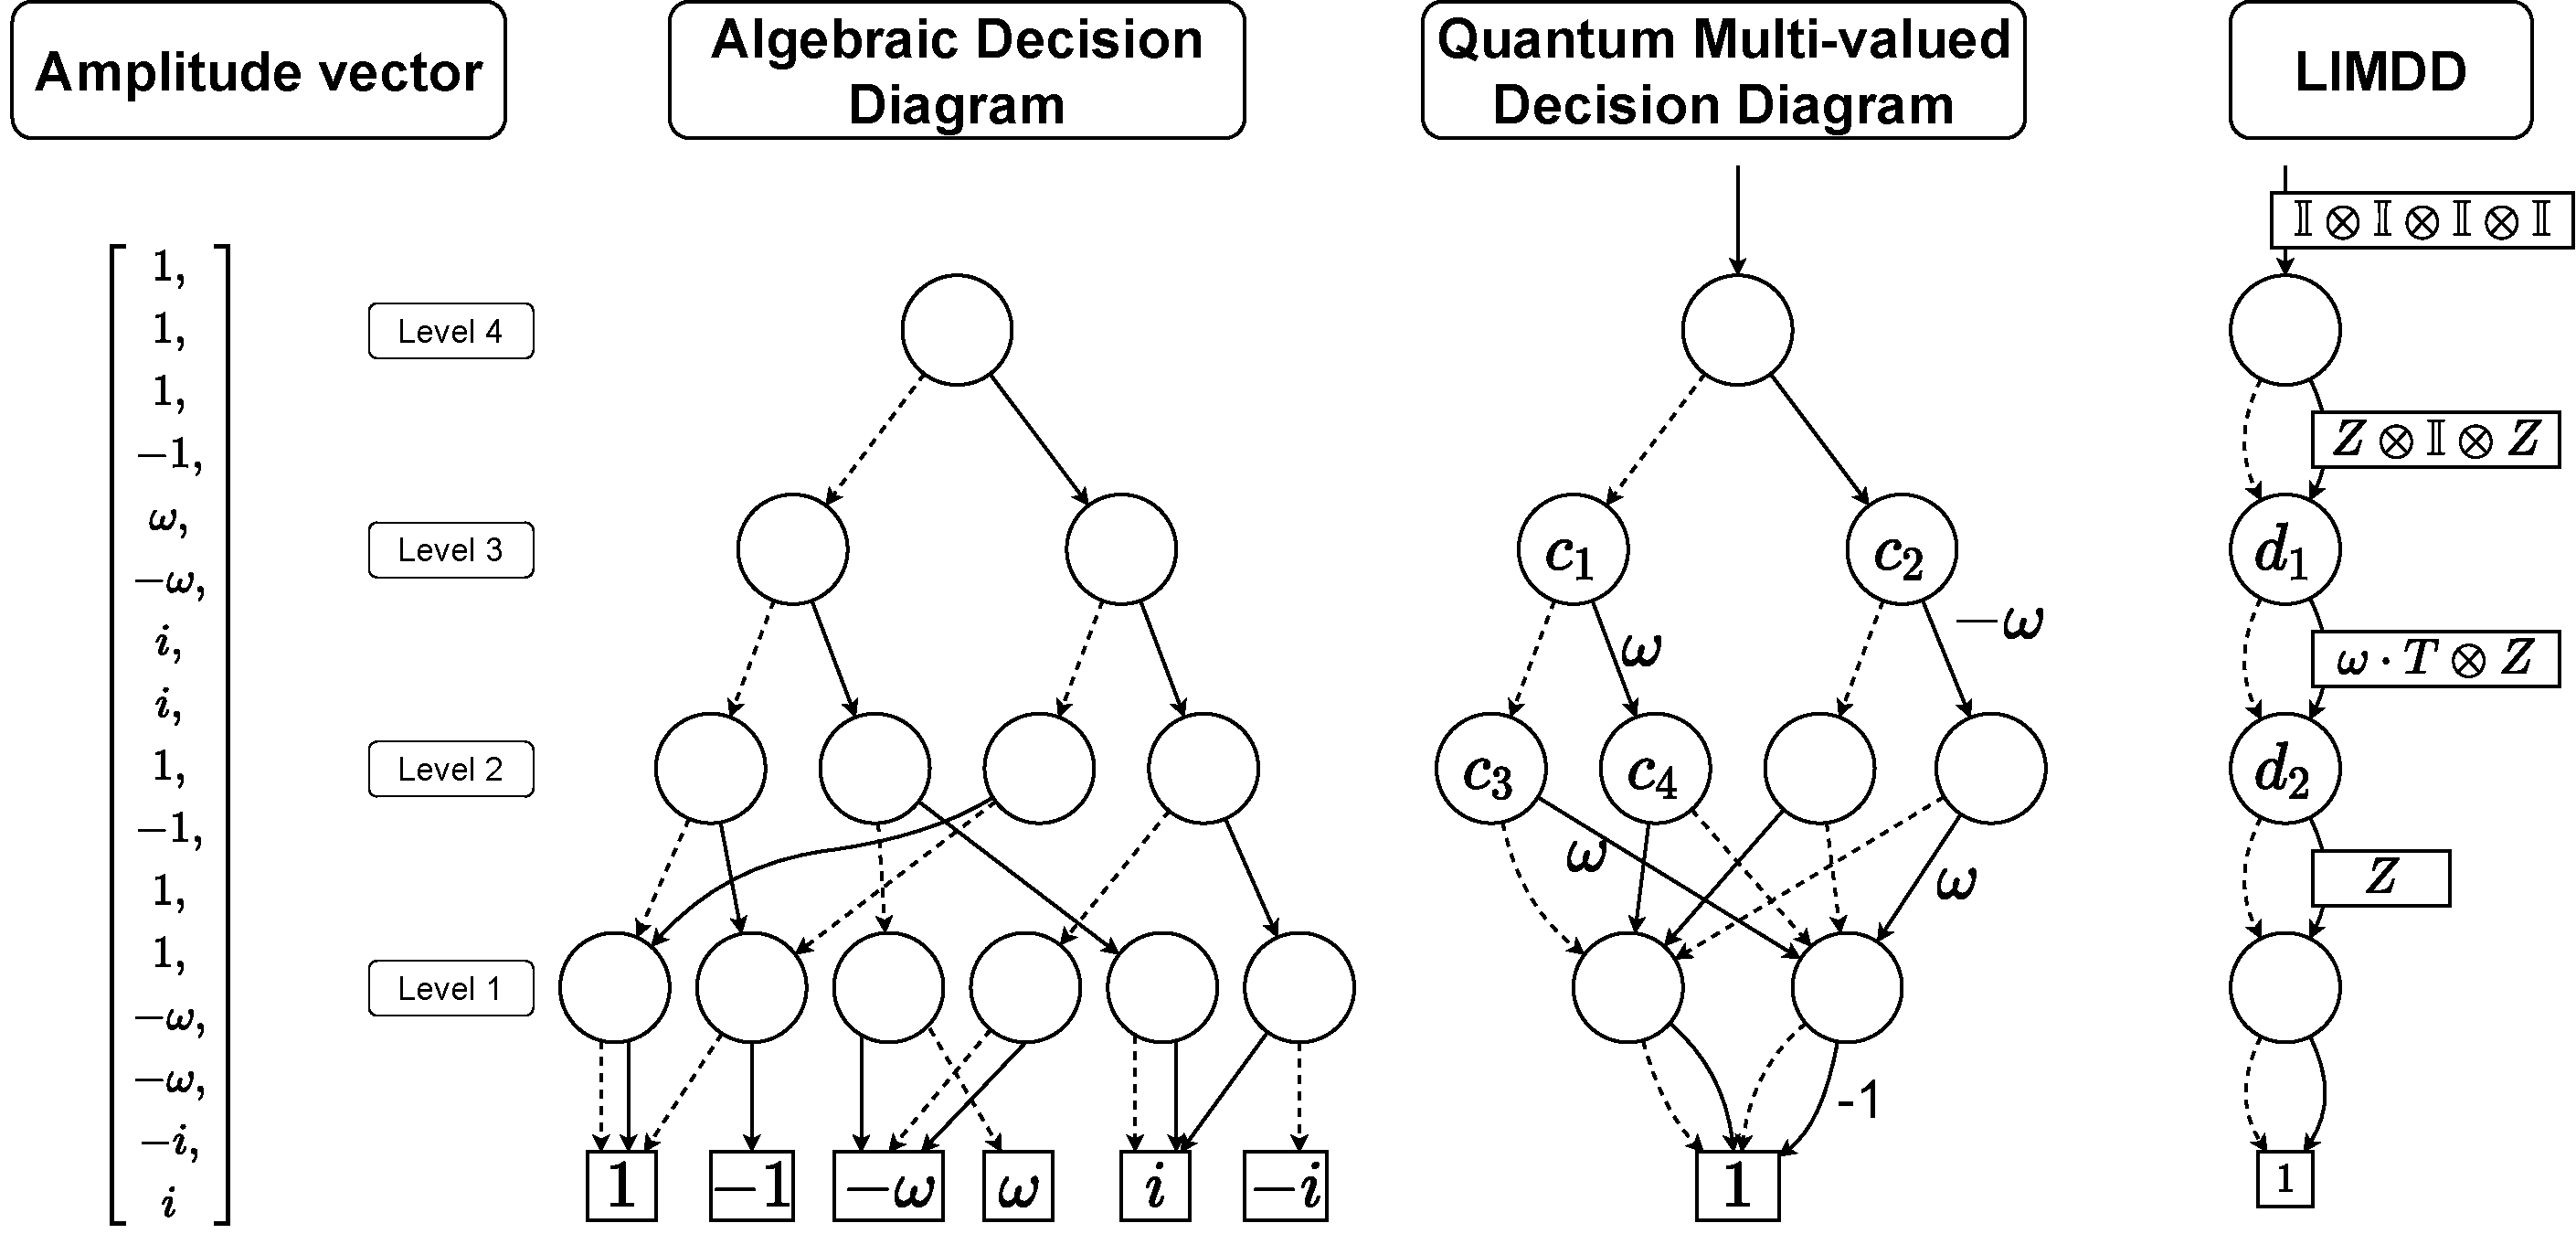
\includegraphics[width=\textwidth]{pics/qmdd-isoqmdd-example-4-qubits-new-notation.pdf}
	\caption{A four-qubit quantum state shown as: an amplitude vector (left), an \add, a \qmdd and a \limdd (right). Diagram nodes are horizontally ordered in `levels' with qubit indices ${4,3,2,1}$.}
	\label{fig:qmdd-isoqmdd-exposition}
\end{figure}

%The formal definition of \limdd is as follows.

\tikzset{every node/.style={initial text={}, inner sep=2pt, outer sep=0}}


\begin{definition}[$G$-\limdd]
	\label{def:limdd}
    An $n$-\glimdd is a rooted, directed acyclic graph (DAG) which represents an $n$-qubit quantum state (or matrix).
    Formally, a \glimdd is a $6$-tuple $(\Node\cup \{\leaf\}, \index,\Low,\High,\lbl,e^r)$,
    where:
\begin{itemize}
	\item $\Node$ is a set of nodes with qubit indices $\index(v) \in [n]$ for $v\in \Node$;
	\item $\Low,\High \colon \Node \to \Node\cup \{\leaf\}$ are the low  and high edge functions;
%	\raisebox{-1mm}{\scalebox{.7}{\tikz{
%		\node[state,minimum size=.2cm] (1) {$v$};
%		\node (-a1) [above left  =.1cm and .3cm of 1] {};
%		\node (-b1) [above right  =.1cm and .3cm of 1] {};
%		\node (1a-) [below left =.1cm and .3cm of 1] {};
%		\node (1b-) [below right = .1cm and .3cm of 1] {};
%		
%		\path[]
%		(-a1) edge node {} (1)
%		(-b1) edge node {} (1)
%		(1) edge node {} (1a-)
%		(1) edge node {} (1b-);
%	}}}.
	\item $\lbl\colon \Low\cup \High\to G$-$\LIM\cup\set 0$ is a function labeling edges with LIMs or $0$;
%       \raisebox{-1mm}{\scalebox{.7}{\tikz{
%            \node[] (1) {};
%            \node [below = .5 of 1] (2) {};
%            \path[] 
%                (1) edge node[right] {$ (\lambda, A_1,\ldots, A_n)$} (2);
%        }}}, and
	\item a root edge $e^r$ without source pointing to root node $r\in \Node$;
%		\raisebox{-1mm}{\scalebox{.7}{\tikz{
%			\node[state,initial,minimum size=.2cm] (r) {$r$}; 
%			\node[below left= .1cm and .3cm of r] (1) {};
%			\node [below right= .1cm and .3cm of r] (2) {};
%			\path[] 
%			(r) edge [dotted] node {} (1)
%			(r) edge [dotted] node {} (2);
%		}}},
    \item a unique leaf node $\leaf$ (a sink) with label $\index(s) = 0$ 
    representing the number $1$;
%        \raisebox{-.5mm}{\scalebox{.7}{\tikz{
%            \node[draw, rectangle,minimum size=.2cm] (s) {$1$}; 
%            \node[above left= .1cm and .3cm of s] (1) {};
%            \node[above= .2cm of s] (a) {};
%            \node [above right= .1cm and .3cm of s] (2) {};
%            \path[] 
%                (1) edge [dotted] node {} (s)
%                (a) edge [dotted] node {} (s)
%                (2) edge [dotted] node {} (s);
%        }}},
%\item If an edge has label $0$, then it points to the leaf node.
%    Otherwise, if $v$ is a node with children $v_0, v_1$, then $\index(v_0) = \index(v_1) = \index(v)-1$;
%        \todo[inline]{note: this used to be the Zero Edges Rule before}
\end{itemize}
Depending on context, we interpret $\lbl(\low v)$ as a node $v_0$ or edge  $(v, v_0)$, etc.
We define the semantics of a (non-leaf) node $v$ and edge $e=(w,v)$  by overloading the Dirac notation:
\begin{align*}
\ket{e} & \defn \begin{cases}
    \lambda \cdot  (\mathcal{Q}_{\index(v)}\otimes \cdots \otimes \mathcal{Q}_1) \cdot \ket v & \text{if $\lbl(e) = (\lambda,  \mathcal{Q}_1, \ldots , \mathcal{Q}_{\index(v)})$} \\
	[0, \dots,0]^\dagger & \text{if $\lbl(e)=0$} \end{cases} \\
\ket{v}     & \defn \ket{0}\otimes\ket{\low v}+ \ket{1}\otimes \ket{\high v}
\end{align*}
\end{definition}

The coefficient $\langle x | e \rangle$ for bitstring $x \in \{0, 1\}^n$ 
of a \limdd with root edge $e$ representing an $n$-qubit state $\ket e$ 
is read by traversing the \limdd from top to bottom according to \autoref{def:limdd}
(i.e., pushing down the LIMs).
It is best illustrated by example, e.g., reading the amplitude for $1111$ in the \limdd of
\autoref{fig:qmdd-isoqmdd-exposition}. The LIM on the root edge is the identity, so we can simply follow the 1-edge to get a new root edge with LIM $P_3\otimes P_2 \otimes P_1 =Z\otimes \id \otimes Z$~to~$d_1$. 
Since the most significant operator ($P_3$) is a $Z$, we multiply the LIM on the 1-edge of $d_1$ (which has $\index(d_1)=3$) with $-1$ and the remainder of the LIM ($\id \otimes Z$),
yielding $ - \omega T \otimes \id$, etc. Eventually the leaf is reached, when only a factor remains (= the sought amplitude).
If we would encounter an $X$ (or $Y$) as $P_3$, we would also have to switch the high (1)
and the low (0) edge, thus taking the 0- instead of 1-edge (and multiply by $-i$ for $P_3 = Y$).
For the choice $G=\Pauli$, this is formalized in the \follow{}{} procedure given in \autoref{sec:quantum-simulation}.

Let us now summarize the representation and manipulation capabilities of the \limdd data structure.
A $G$-\limdd is exact and universal, i.e., for each $n$-qubit quantum state $\ket\phi$ there is a \limdd with root edge $e$ such $\ket e = \ket\phi$, for any choice of parameter $G$.
In particular, a \glimdd with $G=\set{\mathbb I}$ captures all \qmdds by definition.
As all groups $G$ contain the identity operator $\mathbb I$, the universality of \limdds follows from the universality of QMDDs.
Furthermore, for the choice $G=\textsf{Pauli}$, the states that \limdds can represent using polynomial space include all stabilizer states, which is a feature that \qmdds do not posses, as shown in \autoref{sec:exponential-separations}.
Finally, $\textsf{Pauli}$-\limdds can also \emph{manipulate} and measure quantum states, thereby enabling the simulation of quantum circuits, as shown in \autoref{sec:simulation}. 
For many operations, we show that the manipulation is also efficient, i.e., it takes polynomial time in the size of the \limdd representation of the quantum state/circuit.
Specifically, \limdds are often faster than \qmdds, and never slower than a multiplicative factor $O(n^3)$.

From here on, we will focus on the choice $G=\Pauli$, omitting the prefix $\Pauli$- in front of $\limdd$ unless it is clear that we mean otherwise, and hence write $\simeq$ to mean $\simeq_{\textnormal{Pauli}}$.

%From here on, we will focus on the choice $G=\Pauli$, omitting the prefix $\Pauli$- in front of $\limdd$ unless it is clear that we mean otherwise, and hence write $\simeq$ to mean $\simeq_{\textnormal{Pauli}}$.
%For $\Pauli$-\limdds representing an $n$-qubit state $\ket{\phi}$, reading the coefficient $\langle x | \phi\rangle$ of bitstring $x \in \{0, 1\}^n$ is done by traversing the \limdd from top to bottom: at a node with incoming edge label $\lambda P_n \otimes \dots \otimes P_n$, following the $x_k$-edge  if $P_k\ket{x_k} \propto \ket{x_k}$ (e.g. the $0$-edge when $x_k = 0$ and $P_k \in \{\id[2], Z\}$) and the $(1 - x_k)$-edge if $P_k \ket{x_k} \propto \ket{1 - x_k}$ instead (e.g. the $1$-edge when $x_k = 0$ and $P_k \in \{X, Y\}$).
%The coefficient is the product of the factors $\lambda \cdot \langle x_k | P | x_k\rangle$ of the traversed edge labels $\lambda P$.
%For a general group $G$, the coefficients are not encoded in a single path from root to leaf.

%\todo[inline]{Vedran: ok. One may wonder: this is all ok, but how do i compute the amplitude now? It was easy in the QMDD case, I follow the path and multiply numbers...
%	For intuition this is missing for me.
%
%Lieuwe: So do we add an explanation how to compute amplitudes?
%
%Tim: above, I added some text for the case $G=Pauli$, please check.
%}

In general, there are many different $\Pauli$-\limdds which represent a given quantum state.
By imposing a small number of constraints on the diagram, listed in \autoref{def:reduced-limdd} and visualized in \autoref{fig:necessity-of-reduction-rules}, we ensure that every quantum state is represented by a unique `\emph{reduced}' \limdd.
Unique representation, or canonicity, is a useful property of decision diagrams.
In the first place, it allows for circuit analysis and simplification~\cite{bryant1995verification,miller2006qmdd}, by
 facilitating efficient manipulation operations.
In the second place, a reduced diagram is smaller than an unreduced diagram because it merges nodes with the same semantics. For instance, \limdds allow all states in the same $\simeq$ equivalence class to be merged.
The algorithms for quantum circuit simulation in \autoref{sec:quantum-simulation} ensure that all intermediate \limdds are reduced.



%A reduced \limdd representing a state $\ket{\phi}$ has the desirable property that it is the minimum-size diagram among all \limdds representing the state $\ket{\phi}$ (\autoref{thm:reduced-glimdd-minimum-size}).

\begin{definition}[Reduced \limdd]
	\label{def:reduced-limdd}
%	Let $\highlabel,\rootlabel$ and $\beforeq$ be as follows.
%	\begin{itemize}
%		\item The function $\highlabel$ takes as input an $n$-\glimdd node $v$, and outputs an $(n-1)$-$G$-LIM $f(v)$.
%		This function has the property that, if $v$ and $w$ are nodes which satisfy the Low Factoring, Low Precedence and Edge Rules (defined below), and if $\ket{v}\simeq_G\ket{w}$, then $\highlabel(v)=\highlabel(w)$
%		with $\ket v \simeq_G \ket{0}\ket{v_0}+\ket{1}\otimes \highlabel(v)\ket{v_1}$.
%		% and if $\ket{v}=\ket{0}\ket{v_0}+\ket{1}\lbl(\high(v))\ket{v_1}$ then $\ket{v}$ is isomorphic to $\ket{0}\ket{v_0}+\ket{1}\otimes \highlabel(v)\ket{v_1}$.
%		%ALFONS: this seems a corollary of the definition
%		In other words, $\highlabel$ is constant within an isomorphism class.
%		\item The function $\rootlabel$ takes as input a \glimdd{}'s distinguished root edge $e^r$, and outputs a LIM $\rootlabel(e^r)$.
%		This function satisfies the property that, if $e^{r}$ and $e^q$ are the root edges of two \glimdds, and if the root nodes $r$ and $g$ satisfy the reduction rules below except the ``Root edge determinism rule'', and if $\ket{e^r}=\ket{e^q}$, then $\rootlabel(e^r)=\rootlabel(e^q)$.
%		\item $\beforeq$ is a total order on the nodes of the diagram.
%	\end{itemize}
	A \pauli-\limdd is \emph{reduced} when it satisfies the following constraints.
	It is \emph{semi-reduced} if it satisfies all constraints except high determinism.
%	\footnote{}
	\begin{enumerate}
		\item \textbf{Merge: } No two nodes are identical: We say
            two nodes $v,w$ are identical~if $\low v= \low w, \high v = \high w,
                \lbl(\low v)=\lbl(\low w)$, $\lbl(\high v)=\lbl(\high w)$.
		\item \textbf{(Zero) Edge: } Any edge $(v,w) \in \High \cup \Low $
has $\index(v) = \index(w) + 1$, and if $\lbl(v,w)=0$, then both edges point to the same node, i.e., $\high v = \low v = w$.
		\item \textbf{Low Precedence: } For each internal node $v$, we have $\low v \beforeq \high v$, where  $\beforeq$ is a total order on the nodes of the diagram.
		\item \textbf{Low Factoring: } The label on every low edge to a node $v$ is the identity $\id[2]^{\otimes\index(v)}$.
		\item \textbf{High Determinism: } The label on the high edge of any node $v$ is $\highlim =\highlabel(v)$, where $\highlabel$ is a function that takes as input a semi-reduced $n$-{\Pauli}-\limdd node~$v$, and outputs an $(n-1)$-$\Pauli$-LIM $\highlim$
        satisfying
       $\ket v \simeq_{\Pauli} \ket{0}\ket{\low v}+\ket{1}\otimes \highlim\ket{\high v}$.
        Moreover, for any other semi-reduced node $w$ with $\ket{v}\simeq_{\Pauli}\ket{w}$,
         it returns $\highlabel(w) = \highlim$.
		In other words, $\highlabel$ is constant within an isomorphism class.		
%		\item \textbf{Root Edge Determinism: } The label on the root edge is $\rootlabel(e^r)$.
	\end{enumerate}
\end{definition}


\begin{figure}\begin{center}
	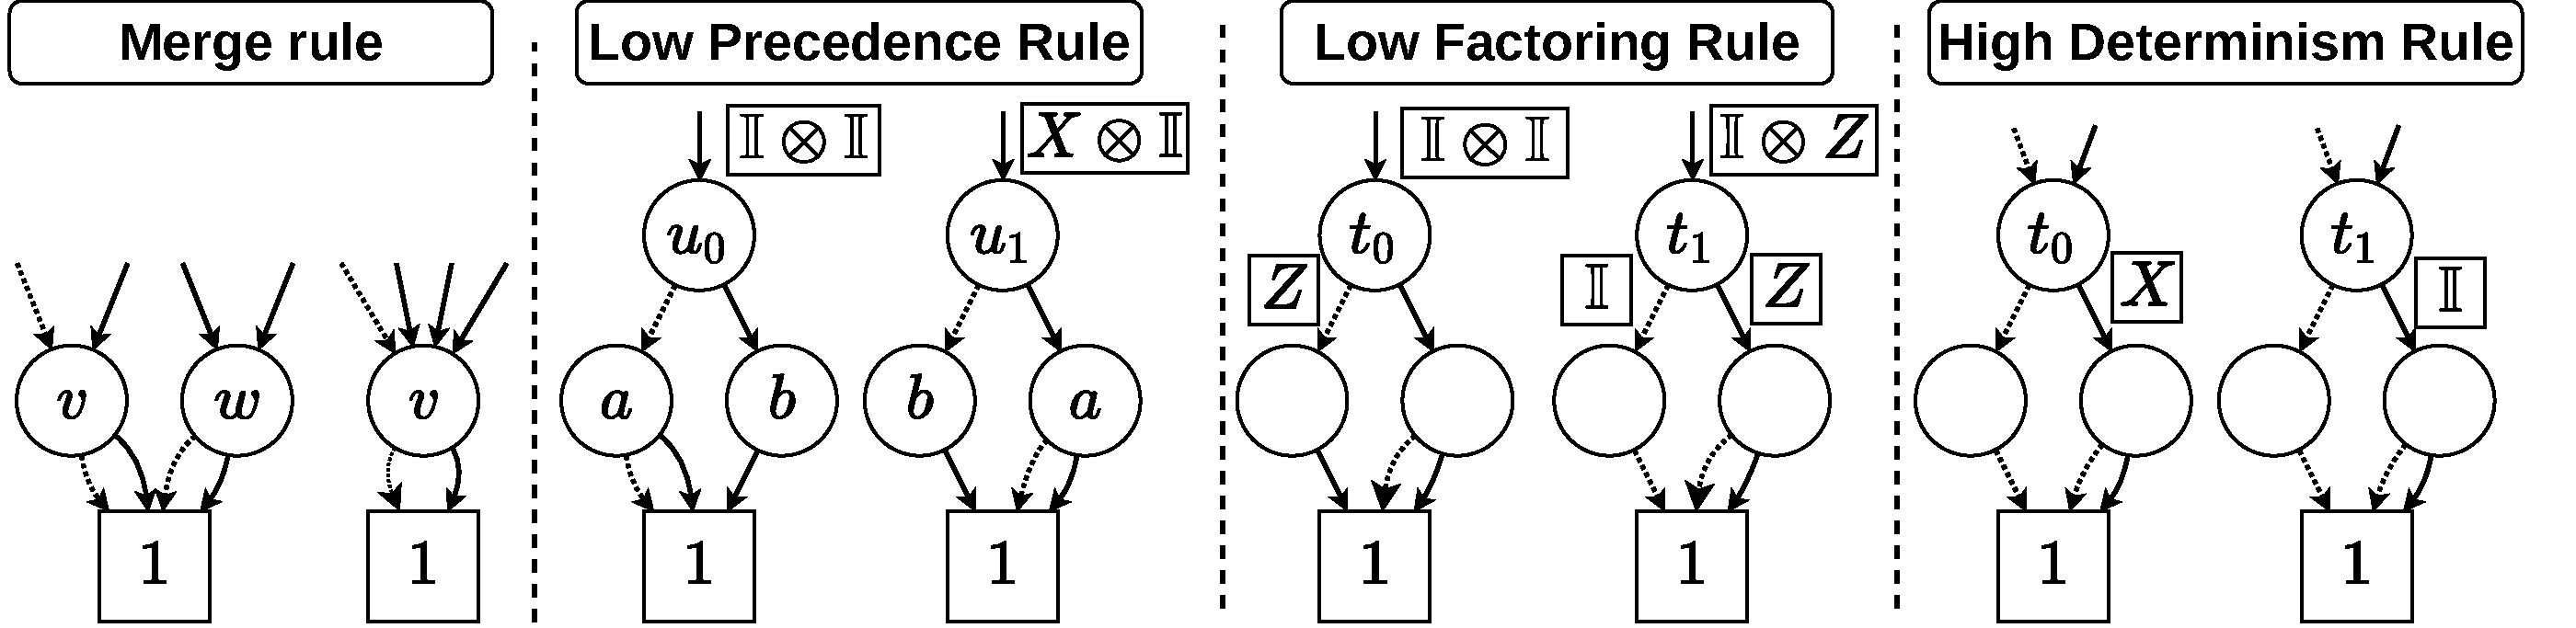
\includegraphics[width=1\textwidth]{pics/necessity-of-reduction-rules.pdf}
	\caption{Illustration of the reduction rules in \autoref{def:reduced-limdd}.
		In each case, the left and right \limdds represent the same state, but the left \limdd violates a reduction rule, while the right \limdd satisfies that rule.
        The Merge rule regards the merging of two identical nodes $v$ and $w$.
		Low Precedence determines which child is the low child, and which is the high child according to~$\beforeq$.
		Low Factoring ensures that the low edge is always labeled with $\mathbb I$.
		High Determinism ensures that the label on high edges is chosen canonically.
		}
	\label{fig:necessity-of-reduction-rules}
\end{center}
\end{figure}

A few observations can be made about the above definition:
	\begin{itemize}
            \setlength\itemsep{1em}
		\item[\namedlabel{obs:nozero}{O1}] There is no reduced \limdd for the $0$-vector, because any low edge must be labeled with~$\id[2]^{\otimes n}$. This is not a problem for us, since the $0$-vector is not a quantum state.
		\item[\namedlabel{obs:knife}{O2}] To represent a state like $\ket{0}\otimes\ket{\phi}$, there is a choice between $\ket{0}\otimes\ket{\phi}$ and $(X\otimes\mathbb I)\ket{1}\otimes \ket{\phi}$.
The low factoring rule forces us to take the $\mathbb I$ label on the low edge, so this gives a node of the form $\ket{0}\otimes \ket{\phi}$. Therefore, the high edge \emph{must} be labeled with $0$. Since, by the zero edges rule, the high edge then points to the same node as the low edge the low precedence rule vacuously holds for such states.
		\item[\namedlabel{obs:subgroups}{O3}] The definition of reduced \limdd cannot always be applied to $G$-\limdd when $G$ is a subgroup of the Pauli group; in particular, such a diagram may not be universal. This is because the low precedence rule requires that $v_0\beforeq v_1$ for every node, so if $G$ is a group which does not contain the $X$, then no reduced \glimdd represents a state $\ket 0 \ket {v_0} + \ket 1 \ket {v_1}$ where $v_1 \beforeq v_0$.
            %In \autoref{sec:exponential-separations}, we come back to this issue.
%            \todo[inline]{Tim: why is this an `issue'? More like a topic, isn't it? Why is it relevant to mention this?}
\item[\namedlabel{obs:delete}{O4}] While the literature on other decision diagrams~\cite{akers1978binary,bryant86,feinstein2011skipped} often considers a ``redundant test'' rule that allows edges to skip multiple levels, we omit this reduction for the sake of simplicity, because it offers only linear improvements in the best case and complicates correctness proofs (see, e.g., \cite[Lemma 1]{andersen1997introduction}). There is however no fundamental reason which would prevent the addition of a similar redundancy reduction.
%	\item[\namedlabel{obs:root-edge}{O5}] the root edge of a diagram may be any LIM; in particular, it is not necessarily equal to $\mathbb I_2^{\otimes n}$.\todo{remove; has nothing to do with reduced.}
%\todo[inline]{This has to be addressed for S4 to work...}
\end{itemize}


\autoref{lemma:node-canonicity-strong} shows that  \limdds are canonical,
in the sense that its nodes 
uniquely represent equivalence classes under $\simeq$ as expressed in \autoref{cor:node-canonicity-strong}. This does not mean that the root edge of a \limdd canonically represents a quantum state. We instead show in \autoref{sec:equality} how to check whether two root edges represent the same state.


%\begin{lemma}
%    [Reduced \limdds have reduced sub-\limdds]
%    \label{lemma:sub}
%    Let $L$ be a \limdd.
%    If the left edge of $v_L$ has label $\unit$, its right edge is labelled $\highlabel(v_L)$ or is labelled zero and points to the same node as its left edge, its children $v_0, v_1$ satisfy Low Precendence, and each node ``under its span'' satisfies the Merge rule, then all these properties also hold for its children.
%\end{lemma}









\begin{corollary}[of \autoref{lemma:node-canonicity-strong}]
    \label{cor:node-canonicity-strong}
    Each equivalence class under $\simeq$, has a unique representative reduced \limdd node $v$, which follows from \autoref{lemma:node-canonicity-strong} and the transitivity of $\simeq$.
\end{corollary}

\begin{lemma}[Node canonicity]
    \label{lemma:node-canonicity-strong}
    For each $n$-qubit state vector $\ket{\phi}$, there exists a unique reduced Pauli-\limdd $L$ with root node $v_L$
    such that $\ket{v_L} \simeq \ket{\phi}$.
%    Isomorphic state vectors are represented by the root node of a unique reduced Pauli-LIMDD.
%    That is, for each state vector $\ket{\phi}$, the set
%    \[
%        C(\ket{\phi}) = \{\textnormal{reduced \limdd L} | \ket{v_L} \simeq \ket{\phi}\}
%    \]
%    satisfies:
%    (a) $C(\ket{\phi}) > 0 $ and (b) $C(\ket{\phi}) \leq 1$.
%    (a) there exists a reduced Pauli-LIMDD $L$ such that $\ket{v_L} \simeq \ket{\phi} \simeq \ket{\psi}$, and
%    : if $\ket{\phi} \simeq \ket{\psi}$, then:
%
%    (b) if there are two reduced Pauli-LIMDDs, with root nodes $v$ and $v'$, then $\ket{v} \simeq \ket{v'} \simeq \ket{\psi}$ implies $v=v'$.
\end{lemma}
\begin{proof}
%	\todo[inline]{From now on, we will write $\simeq$ to mean $\simeq_{\textnormal{Pauli}}$?}
	
    We use induction on on the number of qubits $n$ to show universality (the existence of an isomorphic \limdd node) and uniqueness (canonicity).
%    \todo[inline]{Tim: can't we move proof to appendix?}

%In the lemma's proof, we refer to \limdd DAGs with capitals $L,M$, and their root nodes with $v_L, v_M$.
%Edges to $n$-qubit nodes $v$ in the \limdd carry a Pauli isomorphism $A = \lambda, A_1, \dots, A_n$ according to \autoref{def:limdd}, i.e., a Pauli string interpreted as a LIM $A_n \otimes \dots \otimes A_1$ multiplied by a nonzero complex factor $\lambda$. Note that the factor $\lambda$ can be zero.

    \textbf{Base case.}
    If $n=0$, then $\ket{\phi}$ is a complex number $\lambda$.
    A reduced Pauli-\limdd for this state is the leaf node representing the scalar $1$.
    To show it is unique, consider that nodes $v$ other than the leaf have an $\index(v) > 0$,
    by the edges rule, and hence represent multi-qubit states.
    Since the leaf node itself is defined to be unique, the merge rule is not needed and canonicity follows. Finally, $\ket{\phi}$ is represented by root edge
    $\ledge \lambda1$.
    %
    
    \textbf{Inductive case.}
    Suppose $n>0$.
    We first show existence, and then show uniqueness.
    
    We use the unique expansion of $\ket{\phi}$ as $\ket{\phi} = \ket{0} \otimes \ket{\phi_0} + \ket{1}\otimes \ket{\phi_1}$ where $\ket{\phi_0}$ and $\ket{\phi_1}$ are either $(n-1)$-qubit state vectors, or the all-zero vector.
%    \todo[inline]{Quantum state vectors are defined to be non-zero in \autoref{def:state-vector}, but these vectors are allowed to be zero. -LV}
    We distinguish three cases based on whether $\ket{\phi_0}, \ket{\phi_1} = 0$.

   \textbf{Case $\boldsymbol{\ket{\phi_0}, \ket{\phi_1} = 0}$:}
    This case is ruled out because $\ket{\phi} \neq 0$.

    \textbf{Case $\boldsymbol{\ket{\phi_0}=0}$ or $\boldsymbol{\ket{\phi_1} = 0}$:}
        In case $\ket{\phi_0}\neq 0$,
       by the induction hypothesis, there exists a Pauli-\limdd with root node $w$ satisfying
        $\ket{w} \simeq \ket{\phi_0}$. By definition of $\simeq$,
        there exists an $n$-qubit Pauli isomorphism $A$ such that 
        $\ket{\phi_0} = A \ket{w}$.
       We construct the following reduced Pauli-\limdd for $\ket{\phi}$: 
        $\lnode[v] I{w}0{w}$. 
        In case $\ket{\phi_1}\neq 0$, we do the same for root
            $\ket{w} \simeq \ket{\phi_1} = A \ket w$.
        In both cases, it is easy to check that the root node is reduced.
        Also in both cases, we have $\ket \phi \simeq \ket v$ because 
        either $\ket \phi = \id[2] \otimes A \ket v$ or 
        $\ket \phi = X \otimes A \ket v$ as illustrated in \autoref{fig:reduced1} (left).

\begin{figure}
\tikz[->,>=stealth',shorten >=1pt,auto,node distance=1.5cm,
        thick, state/.style={circle,draw,inner sep=0pt,minimum size=18pt}]{
    \node[state] (1) {$v'$};
    \node[above = .5cm of 1,xshift=1.55cm,fill=black] (x) {};%{$\ket \phi$};
    \node[state] (1a) [below = 1cm of 1, xshift=1.7cm] {$w$};
    
    \path[]
    (x) edge[bend left=-20]     node[above left,pos=.7] {$\id[2]^{\otimes n}$} (1)
    (1) edge[e0,bend left=-20] node[pos=.1,left] {$A$} (1a)
    (1) edge[e1,bend right=-20] node[pos=.1,above right] {$0$} (1a)
    ;

    \node[state, right = 2.5cm of 1] (2) {$v$};
%    \node[above = .5cm of 2] (x)  {$\ket \phi$};%{$= \id[2] \otimes A \ket{v}$};
    \path[]
    (x) edge[bend left=20]     node[above right,pos=.7] {$\id[2] \otimes A$} (2)
    (2) edge[e0,bend left=-20] node[pos=.1,left] {$\id[2]^{\otimes n}$} (1a)
    (2) edge[e1,bend right=-20] node[pos=.2,right] {$0$} (1a)
    (1) --  node[yshift=.1cm] {$\rightsquigarrow$} (2)
    ;
    }~~~~~~~~~~~~~~~
\tikz[->,>=stealth',shorten >=1pt,auto,node distance=1.5cm,
        thick, state/.style={circle,draw,inner sep=0pt,minimum size=18pt}]{
%    \node[above = .5cm of 1] (x) {$\ket \phi$};
    \node[state] (1) {$v''$};
    \node[state] (1a) [below = 1cm of 1, xshift=2.3cm] {$v_L$};
    \node[state] (1b) [below = 1cm of 1, xshift=3.8cm] {$v_R$};
    \path[]
    (1) edge[e0] node[pos=.1,left] {$A$} (1a)
    (1) edge[e1] node[pos=.1,above right] {$B$} (1b)
    (1a) --  node[yshift=-.2cm] {$\beforeq$} (1b)
    ;

    \node[state, right = 2.5cm of 1] (2) {$v'$};
    \node[above = .5cm of 2,fill=black] (x)  {};%{$= \id[2] \otimes A \ket{v'}$};
    \path[]
    (x) edge[bend left=-20]     node[above left,pos=.8] {$\id[2]^{\otimes n}$} (1)
    (x) edge     node[right,pos=.4] {$\id[2] \otimes A$} (2)
    (2) edge[e0] node[pos=.2,left] {$\id[2]^{\otimes n}$} (1a)
    (2) edge[e1] node[pos=.1,right] {$ A^{-1}B$} (1b)
    (1) --  node[yshift=.1cm] {$\rightsquigarrow$} (2)
    ;
    
    \node[state, right = 2.5cm of 2] (3) {$v$};
%    \node[above = .5cm of 3] (x)  {}; %{$ =  (\id[2] \otimes A)\rootlim \ket{v}$};
    \path[]
    (x) edge[bend left=20]      node[above right,pos=.8] {$(\id[2] \otimes A)\rootlim$} (3)
    (3) edge[e0] node[pos=.1,above left] {$\id[2]^{\otimes n}$} (1a)
    (3) edge[e1] node[pos=.2,below right] {$\highlim$} (1b)
    (2) --  node[yshift=.1cm] {$\rightsquigarrow$} (3)
    ;
    }
	\caption{Reduced node construction in case $\ket{\phi_1} = 0$ (left), and
	        $\ket{\phi_0}, \ket{\phi_0} \neq 0$ and $v_L \beforeq v_R$ (right).
	        For cases $\ket{\phi_0} = 0$ and $v_R \beforeq v_L$, we take instead root edge $ X \otimes A$ and swap low/high edges.
	        The black square (\scalebox{.7}{$\blacksquare$})
	        signifies a unique quantum state (all root edge represent this one state).
%            \todo[inline]{Tim: why do we need to show the state above each node? Aren't these obvious from the figure? (i.e. each state is of the form $(rootedge) \ket{rootnode}$}
            }
	\label{fig:reduced1}
\end{figure}

 
    \textbf{Case $\boldsymbol{\ket{\phi_0}, \ket{\phi_1} \neq 0}$:}
    By the induction hypothesis, there exist \pauli-\limdds $L$ and $R$ with root nodes
    $\ket{v_{L}} \simeq \ket{\phi_0}$ and $\ket{v_{R}} \simeq \ket{\phi_1}$.\footnote{Note that the induction hypothesis implies a `local' reduction of \limdds $L$ and $R$, but not automatically a reduction of their union. For instance, $L$ might contain a node $w$ and $R$ a node $w$ such that $v \simeq w$. While the other reduction rules ensure that $v$ and $w$ will be structurally the same, the induction hypothesis only applies the merge rule $L$ and $M$ in isolation, leaving two separate identical nodes $v,w$.
We can solve this by applying merge on the union of nodes in $L$ and $M$, to merge any equivalent nodes.}
    By definition of $\simeq$, there exist $n$-qubit Pauli isomorphisms $A$ and $B$ such that $\ket{\phi_0} = A \ket{v_{L}}$ and $\ket{\phi_1} = B \ket{v_{R}}$.
    In case $v_{L} \beforeq v_{R}$,
       we construct the following reduced Pauli-\limdd for $\ket{\phi}$: the root node is $\lnode[v] {\mathbb I}{v_{L}}E{v_{R}}$, where
    $E$ is the LIM computed by $\highlabel(\lnode{\mathbb I}{v_L}{A^{-1}B}{v_R})$ . 
    Otherwise, if $v_{R}\beforeq v_{L}$, then we construct the following reduced Pauli-\limdd for $\ket{\phi}$: the root node is $\lnode[v] I{v_{R}}F{v_{L}}$, where $F=\highlabel(\lnode{\mathbb I}{v_L}{B^{-1}A}{v_R})$.
    It is straightforward to check that, in both cases, this Pauli-\limdd is reduced.
    Moreover, $\ket v$ isomorphic to $\ket \phi$ 
    as illustrated in \autoref{fig:reduced1} (right).



    To show uniqueness, let $L$ and $M$ be reduced \limdds (root nodes $v_L, v_M$) such that $\ket{v_L} \simeq \ket{\phi} \simeq \ket{v_M}$.
    \def\Ptop{P_{\textnormal{top}}}
    \def\Prest{P_{\textnormal{rest}}}
    Expanding the semantics of $v_L$ and $v_M$, this implies there exists a Pauli isomorphism $\lambda \Ptop \otimes \Prest \neq 0$, where $\Ptop$ is a single-qubit Pauli and $\Prest$ an $(n-1)$-qubit Pauli isomorphism, such that
        \begin{align}
        \label{eq:canonicity-equation-1}
       \lambda \Ptop \otimes \Prest (\ket{0} \otimes A_L \ket{v_L^0} + \ket{1} \otimes B_L \ket{v_L^1})
        =
        \ket{0} \otimes A_M \ket{v_M^0} + \ket{1} \otimes B_M \ket{v_M^1}
        .
        \end{align}

    
    We distinguish two cases from here on: where $\Ptop \in \{\unit, Z\}$ or $\Ptop \in \{X,  Y\}$.
    
    \textbf{Case $\boldsymbol{\Ptop = I,Z}$.}
    If $\Ptop = \diag z$ for $z \in \{1, -1\}$,  then
    \autoref{eq:canonicity-equation-1} gives:
%        \begin{align}
%        \label{eq:canonicity-equation-1}
%       \ket{0} \otimes \lambda\Prest A_L \ket{v_L^0} + \ket{1} \otimes z \lambda\Prest B_L \ket{v_L^1}
%=
%\ket{0} \otimes A_M \ket{v_M^0} + \ket{1} \otimes B_M \ket{v_M^1}
%        \end{align}
        \begin{align}
        \label{eq:canonicity-equation-2}
            \lambda \Prest A_L \ket{v_L^0} = A_M \ket{v_M^0}
            \qquad\textnormal{and}\qquad
            z\lambda \Prest B_L \ket{v_L^1} = B_M \ket{v_M^1}
        \end{align}
            By low factoring, we have $A_L = A_M = \unit$, so we obtain
$ \lambda  \Prest \ket{v_L^0} = \ket{v_M^0}$.      
        Hence $\ket{v_L^0}$ is isomorphic with $\ket{v_M^0}$, so by induction hypothesis and
         \autoref{cor:node-canonicity-strong}, we have $v_L^0 = v_M^0$. 
         We now show that also $v_L = v_M$ by considering two cases.
\begin{description}
        \item[$B_L \neq 0$ and $B_M \neq 0$:] then $z\lambda \Prest B_L\ket{v_L^1}=B_M\ket{v_M^1}$, so the nodes $v_L^1$ and $v_M^1$ represent isomorphic states, so by the induction hypothesis  and \autoref{cor:node-canonicity-strong} we have $v_L^1=v_M^1$.
        We already noticed by the low factoring rule that $v_L$ and $v_M$ have $\mathbb I$ as low edge label.
        By the high edge rule, their high edge labels are $\highlabel(v_L)$ and $\highlabel(v_M)$, and since the reduced \limdds $L$ and $M$ also satisfy low precedence and edge rules and $\ket{v_L} \simeq \ket{v_M}$, we have $\highlabel(v_M) = \highlabel(v_L)$ by definition of $\highlabel$.

        \item[$B_L = 0$ or $B_M= 0$:] In case $B_L = 0$,
        %, then since no state vector has norm 0, we find that $B_M = 0$.
        we see from \autoref{eq:canonicity-equation-2} that $0=B_M\ket{v_M^1}$.
        Since the state vector $\ket{v_M^1}\ne 0$ by \ref{obs:nozero}, it follows that $B_M=0$.
        Otherwise, if $B_M=0$, then \autoref{eq:canonicity-equation-2} yields $z\lambda\Prest B_L\ket{v_L^1}=0$.
        We have $z \lambda\ne 0$, $\Prest \ne 0$ by definition, and $\ket{v_L^1}\ne 0$ by \ref{obs:nozero}.
        Therefore $B_L=0$. In both cases, $B_L=B_M$.
%        Let's first assume $B_L \neq 
\end{description}
        We conclude that in both cases $v_L$ and $v_M$ have the same children and the same edge labels, so they are identical by the merge rule.

        \textbf{Case $\boldsymbol{\Ptop = X, Y}$.}
    If $\Ptop = \begin{smallmat}0 & z^* \\ z & 0\end{smallmat}$ for $z \in \{1, i\}$, then
    \autoref{eq:canonicity-equation-1} gives:
%        \[
%        \ket{1} \otimes z \Prest A_L \ket{v_L^0} + \ket{0} \otimes z \Prest B_L \ket{v_L^1}
%        =
%        \ket{0} \otimes A_M \ket{v_M^0} + \ket{1} \otimes B_M \ket{v_M^1}
%        \]
        \[
            \lambda z\Prest A_L \ket{v_L^0} = B_M \ket{v_M^1}
            \qquad\textnormal{and}\qquad
            \lambda z^*\Prest B_L \ket{v_L^1} = A_M \ket{v_M^0}
            .
        \]
        By low factoring, $A_L = A_M = \unit$, so we obtain 
        $z\lambda  \Prest \ket{v_L^0} = B_M \ket{v_M^1}$
        and
        $\lambda z^*\Prest B_L \ket{v_L^1} = \ket{v_M^0}$.
To show that $v_L = v_M$, we consider two cases.       
\begin{description}
        \item[$B_L \neq 0$ and $B_M \neq 0$:] we find $\ket{v_L^0} \simeq \ket{v_M^1}$ and $\ket{v_L^1} \simeq \ket{v_M^0}$, so by the induction hypothesis, $v_L^0= v_M^1$ and $v_L^1= v_M^0$.
        By low precedence, it must be that $v_L^1 = v_M^1 = v_L^0 = v_M^0$.
        Now use high determinism to infer that $B_L = B_M$ as in the ${\Ptop = I,Z}$ case.
%(NOTE: THIS IS THE SAME CASE AS Case-IZ \& $B_{\Box}$ nonzero. So this is where the root edge rule will help us choose $P=\Ptop \otimes \Prest$)\todo{I don't follow. Root Edge should not be relevant here.}

        \item[$B_L = 0$ or $B_M = 0$:]
       This case leads to a contradiction and thus cannot occur.
        $B_L$ cannot be zero, because then $\ket{v_M^0}$ is the all-zero vector, which we excluded by \ref{obs:nozero}.
        The other case: $B_M = 0$, then it must be that $\Prest$ is zero, hence $\ket{v_M^0}$ is the all-zero vector, which is again excluded.
\end{description}
 We conclude that $v_L$ and $v_M$ have the same children and the same edge labels  for all choices of $\Ptop$, so they are identical by the merge rule.
\end{proof}

%\begin{corollary}[Canonicity]
%    For each $n$-qubit state vector $\ket{\phi}$, there exists a unique Pauli-LIMDD $L$ such that $\ket{e^L} = \ket{\phi}$.
%\end{corollary}
%\begin{proof}
%    By Lemma~\ref{lemma:node-canonicity-strong}, there exists a unique Pauli-LIMDD $M$ such that $\ket{\phi} \simeq \ket{v_M}$.
%    Denote by $P$ a Pauli isomorphism mapping $\ket{v_M}$ to $\ket{\phi}$.
%    As root edge label, we use $\rootlabel(P\cdot e^{v_M})$.
%    By definition of $\rootlabel$, this label choice is unique.
%\end{proof}


%\newpage
%\newpage
%\newpage


% todo the others

%\autoref{thm:limdd-canonicity-root-edge} shows that for every quantum state $\ket{\phi}$, there is indeed a unique reduced \glimdd whose root edge represents $\ket{\phi}$.
%This implies canonicity, since by \autoref{def:limdd}, every \glimdd represents exactly one quantum state.
%
%\todo[inline]{Theorem does not use low precedence, so it is either incorrect or Def 3 is.}
%
%
%%\todo[inline]{Insert figure which shows that, if the reduction rules are NOT obeyed, then we can get multiple diagrams which represent the same state.}
%\begin{figure}[b]
%	\centering
%	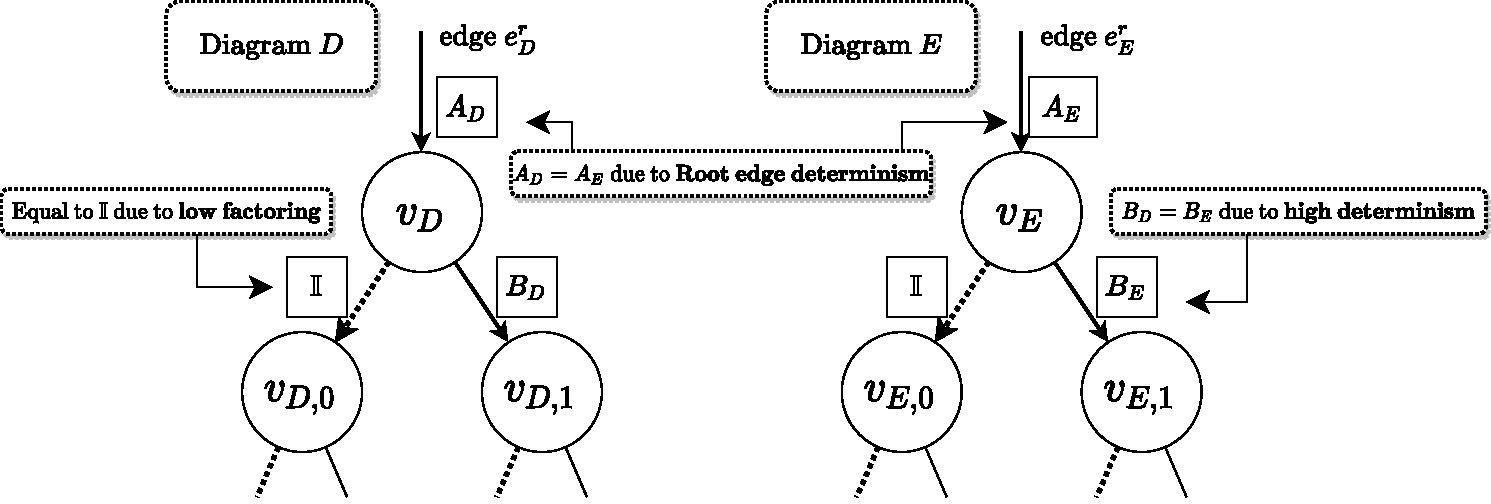
\includegraphics[width=.7\textwidth]{pics/canonicity-two-diagrams.pdf}
%	\caption{Two \glimdds on $n+1$ qubits.}
%	\label{fig:canonicity-two-diagrams}
%\end{figure}
%\begin{theorem}[Canonicity of \glimdd nodes]
%	\label{thm:limdd-canonicity-nodes}
%	If two reduced \glimdd nodes $v_D$ and $v_E$ represent the same state $\ket{v_D}=\ket{v_E}$, and if $G$ is a subgroup of the Dihedral Torus\todo{TODO: Change to Pauli group, or explain exception}, then they are the same diagram.
%\end{theorem}
%\begin{proof}
%	The proof is by induction on the number of qubits.
%	The induction hypothesis is that the theorem holds for all \glimdd nodes on $n$ qubits.
%	
%	\textbf{Base case: $n=0$ qubits. } 
%	There is only one node on $0$ qubits, namely the leaf, representing the scalar $1\in \mathbb C$.
%	Hence, the theorem trivially holds in this case.
%	
%	\textbf{Induction case: $n+1$ qubits. }
%	%	Let $\ket{\phi}$ be a state of $n+1$ qubits, and suppose that two \glimdds $D$ and $E$ represent this state, with $D=(V_D,Low_D,High_D,\textsf{label}_D,e_D^r)$ and $E=(V_E,Low_E,High_E,\textsf{label}_E,e_E^r)$.
%	Suppose that nodes $v_D$ and $v_E$ represent the same $n+1$-qubit state, i.e., $\ket{v_D}=\ket{v_E}$.
%	\alfons{Since $\index(v_D), \index(v_E) = n+1 > 0$, these nodes cannot be leaves.}
%	Hence $v_D$ and $v_E$ are both nodes representing the most significant qubit $n+1$, as implied by the (zero) edges rule\todo{actually requires a few reasoning steps, or we should make it part of the IH},
%	as in \autoref{fig:canonicity-two-diagrams}.
%	%	Say that the diagrams $D$ and $E$ are as in \autoref{fig:canonicity-two-diagrams}.
%	%	In this Figure, the edges $e_D^r$ and $e_E^r$ are labeled with $A_D=\textsf{label}_D(e_D^r)$ and $A_E=\textsf{label}_E(e_E^r)$, and they point to the root nodes $v_D$ and $v_E$, respectively.
%	The node $v_D$ has two (not necessarily distinct) children, $v_{D,0}$ (low) and $v_{D,1}$ (high), and node $v_E$ has children $v_{E,0}$ and $v_{E,1}$.
%	The high edges of nodes $v_D$ and $v_E$ are labeled with $n$-$G$-LIMs $B_D$ and $B_E$, respectively.
%	
%	Since the diagrams $D$ and $E$ are reduced, they satisfy the \emph{Low Factoring}; therefore, the labels on the low edges are $\textsf{label}_D(v_D,v_{D,0})=\textsf{label}_E(v_E,v_{E,0})=\mathbb I$.
%	We show that this implies that $\ket{v_{D,0}}=\ket{v_{E,0}}$.
%	Namely, consider the equation $\ket{v_D}=\ket{v_E}$, and expand the most significant qubit, as follows,
%	\begin{align}
%	\ket{v_D}=\ket{0}\ket{v_{D,0}}+\ket{1}B_D\ket{v_{D,1}} = \ket{0}\ket{v_{E,0}}+\ket{1}B_E\ket{v_{E,1}} = \ket{v_E}
%	\end{align}
%	Since $\ket{0}\ket{v_{D,0}}=\ket{0}\ket{v_{E,0}}$, it follows that $\ket{v_{D,0}}=\ket{v_{E,0}}$.
%	Therefore, by the induction hypothesis, the low children $v_{D,0}$ and $v_{E,0}$ are in fact the same node.
%	
%	
%	The nodes $v_{D}$ and $v_E$ satisfy the \emph{High Determinism Rule}; therefore, the labels on their high edges are equal: $B_D=B_E=\highlabel(v_D)$, because the $\highlabel$ function is constant for nodes representing states in the same equivalence class according to \ref{def:reduced-limdd} and $\ket{v_{D}} = \ket{v_E} \implies \ket{v_{D}} \simeq \ket{v_E}$.
%	%In particular, if $\ket{v}=\ket{0}\ket{v_0}+\ket{1}\lbl(\high(v))\ket{v_1}$ then $\ket{v}$ is isomorphic to $\ket{0}\ket{v_0}+\ket{1}\otimes \highlabel(v)\ket{v_1}$.
%	
%	%\todo{connect to new formalism. Formalize that \highlabel is constant in this case and explain here.}
%	
%	It remains to show that we have $v_{D,1}=v_{E,1}$.
%	To this end, we distinguish two cases: a ``knife'' case, in which $\ket{v_D}=\ket{0}\ket{v_{D,0}}$, and a ``fork'' case.
%	
%	\textbf{Case 1: Knife. }
%	By \autoref{def:reduced-limdd} we have $B_D=B_E=0$.
%	By the zero edge rule, we must have $v_{D,1}=v_{D,0}$ and $v_{E,1}=v_{E,0}$; therefore, we also conclude $v_{D,1}=v_{E,1}$.
%	From the merge rule, we then conclude that the \glimdds $v_D$ and $v_D$ are the same.
%	
%	\textbf{Case 2: Fork. }
%	Since the nodes $v_D$ and $v_E$ represent the same state, consider again the equation $\ket{v_D}=\ket{v_E}$, knowing that $B_D=B_E$:
%	\begin{align}
%	\ket{v_D}=\ket{0}\ket{v_{D,0}}+\ket{1}A_D\ket{v_{D,1}} = \ket{0}\ket{v_{D,0}}+\ket{1}A_D\ket{v_{D,1}} = \ket{v_E}
%	\end{align}
%	It follows that $\ket{1}A_D\ket{v_{D,1}}=\ket{1}A_D\ket{v_{E,1}}$; therefore, in particular $A_D\ket{v_{D,1}}=A_D\ket{v_{E,1}}$.
%	Multiplying both sides with $A_D^{-1}$, we get $\ket{v_{D,1}}=\ket{v_{E,1}}$, i.e., the nodes $v_{D,1}$ and $v_{E,1}$ represent the same state.
%	Therefore, by the induction hypothesis, they must be the same node.
%\end{proof}
%\begin{corollary}
%	\label{thm:limdd-canonicity-root-edge}
%	If root edges $e_D^r, e_E^r$ of reduced \glimdds represent the same state $\ket{e_D^r}=\ket{e_E^r}$, and if $G$ is a subgroup of the Dihedral Torus\todo{tricky}, then they are the same diagram.
%\end{corollary}
%\begin{proof}
%	Since the diagrams $D$ and $E$ are reduced, they satisfy the \emph{Root Edge Determinism Rule}.
%	This means that the labels are chosen as $A_D=\rootlabel(\ket{e_D^r})$ and $A_E=\rootlabel(\ket{e_E^r})$.
%	However, because the diagrams represent the same state, i.e., $\ket{e_D^r}=\ket{e_E^r}$, it follows that $A_D=A_E$, i.e., these two root edges have the same label.
%	
%	It follows that the states represented by the nodes $v_D$ and $v_E$ are the same.
%	Namely, since we have $\ket{e_D^r}=\ket{e_E^r}$, and $\ket{e_D^r}=A_D\ket{v_D}$, and $\ket{e_E^r}=A_D\ket{v_E}$, it follows that $A_D\ket{v_D}=A_D\ket{v_E}$, so, multiplying both sides with $A_D^{-1}$, we get $\ket{v_D}=\ket{v_E}$.
%	By \autoref{thm:limdd-canonicity-nodes}, since the two nodes $v_D$ and $v_E$ represent the same state, they are the same nodes.
%	
%	Because the two \glimdds have the same structure below the root nodes, and have the same label on the root edge, we conclude that they are the same diagram.
%\end{proof}



















